\documentclass{article}
\usepackage[utf8]{inputenc}
\usepackage[spanish]{babel}
\usepackage{listings}
\usepackage{graphicx}
\graphicspath{ {images/} }
\usepackage{cite}

\begin{document}

\begin{titlepage}
    \begin{center}
        \vspace*{1cm}
            
        \Huge
        \textbf{Analisis Parcial II - Informatica II.}
            
        \vspace{0.5cm}
        \LARGE
            
        \vspace{1.5cm}
            
        \textbf{Luis Miguel Gil Rodriguez.}
        \\
        \textbf{Maverick Sossa Tobon.}
        \vfill
        \vspace{0.8cm}
            
        \Large
        Despartamento de Ingeniería Electrónica y Telecomunicaciones\\
        Universidad de Antioquia\\
        Medellín\\
        Septiembre de 2021
            
    \end{center}
\end{titlepage}
\tableofcontents
\newpage
\section{Sección introductoria} \label{intro}
En este documento, podremos encontrar las ideas para abordar el parcial numero dos del curso Informatica II. Encontraremos en el detalles tales como el lgoritmo de redimensionamiento de imagenes para luego se mostrados en una martriz de LEDs de un tamaño ce 16 por 16 LEDs.
\section{Analisis del Problema} \label{analisis}
Aqui va la el analisis :)
\section{Algoritmo} \label{algoritmo}
Aqui va la descripcion del algoritmo :)
\section{Circuito.} \label{circuito}
Para la implementación del circuito en la plataforma Tinkercad, primeramente se comenzaron a realizar ensayos con una tira de 16 Neopixeles, la cual se conecta de la siguiente manera:
\begin{enumerate}
  \item La primera fila se conecta al puerto 2 del Arduino
  \item Se le suministra potencia de 5 Voltios a la tira de Neopixel procedentes del Arduino
  \item Se conecta el polo a tierra procedente del Arduino a la tira de Neopixel.
\end{enumerate}
\begin{figure}[h]
  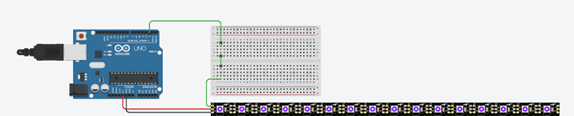
\includegraphics[width=10cm]{figura_1.png}
  \centering
  \caption{Prender fila numero uno de la matriz.}
  \label{fig:fila_uno}
\end{figure}
Se comenzó la etapa de pruebas con la tira de Neopixel, ejemplo de algunas pruebas que se realizaron:
\begin{enumerate}
    \item Cómo prender un Neopixel en específico.
    \item Cómo mostrar un patrón en una tira (ejemplo: Solo prender las posiciones impares, solo prender las posiciones pares).
    \item Cómo prender todos los leds e a la vez.
\end{enumerate}
Una vez superada esta etapa de prueba se agregaron las 15 filas restantes, para obtener una especie de matriz de 16 X 16, en primer lugar se realiza la conexión desde la fila uno hasta la fila cinco de la siguiente manera:
\begin{enumerate}
    \item Se conecta entrada de la fila N con la entrada de la fila N+1.
    \item Se conecta la potencia de la fila N con la potencia de la fila N+1.
    \item Se conecta la tierra de la fila N con la tierra de la fila N+1.
\end{enumerate}
Al intentar interactuar con la matriz, por ejemplo prender una Neopixel en específico se evidencio que tenía un comportamiento de prender por columnas, conducta para nada esperada.\\
\begin{figure}[h]
  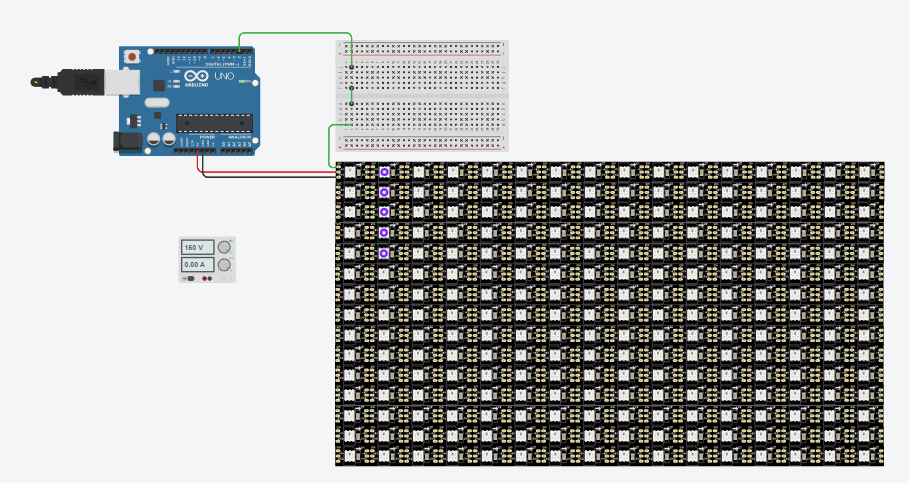
\includegraphics[width=10cm]{figura_2.png}
  \centering
  \caption{Comportamiento no esperado.}
  \label{fig:por_columnas}
\end{figure}
Al evidenciar este comportamiento, de inmediato se repiensa la manera de como realizar satisfactoriamente la conexión. Hasta que se llego hasta la siguiente idea:
\begin{enumerate}
    \item Se conecta salida de la fila N con la entrada de la fila N+1.
    \item Se conecta la potencia de la fila N con la potencia de la fila N+1.
    \item Se conecta la tierra de la fila N con la tierra de la fila N+1.
\end{enumerate}
Luego de haber realizado dicha conexión, se comenzó una nueva etapa de pruebas con el mismo, se intento prender todas las filas conectas, un Neopixel en específico y por último un patrón sencillo, como prender solo las posiciones impares, la diagonal principal de la matriz entre otras pruebas.

\centering
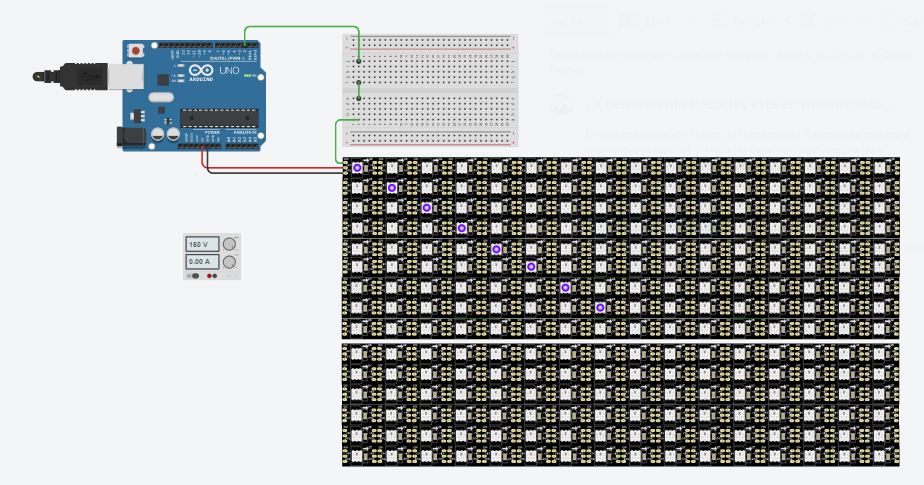
\includegraphics[width=8cm]{figura_3.png}
  
A continuacion se mostrara el circuito desarrollado, cabe mencionar, que el aspecto que aqui se muestra no sera el definiticvo, pues se reorganizaran las tiras de Neopixel de una manera mas estetica.

\centering
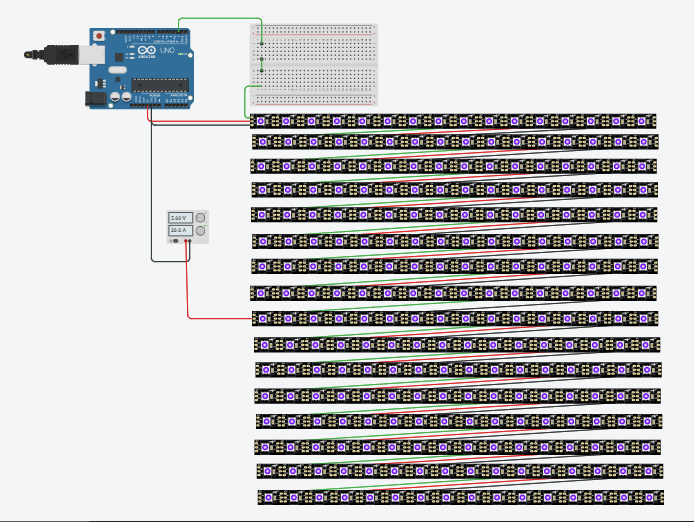
\includegraphics[width=8cm]{figura_4.png}

\begin{enumerate}
    \item Los cables de color verde se encargan de llevar los datos a la matriz de LEDs
    \item Los cables de color Negro representan la el Polo a Tierra.
    \item Los cables de color Rojo representan la potencia (5.0 V).
    \item Se conecta un suministro de energia, el cual alimentara la matriz de LEDs, es decir suministrara potencia a partir de la fila 9 de nuestra matriz. El suministro de energia suministra 5.0 Voltios a la matriz de LEDs.
\end{enumerate}
\bibliographystyle{IEEEtran}
\bibliography{references}
\end{document}

